\documentclass[a4paper]{dnd5}

%\pagestyle{fancy}

\usepackage{wrapfig}

\newcommand\inc[1]{
 \includegraphics[width=0.22\textwidth, height=0.22\textwidth]{#1}
}

\begin{document}
\section*{Historia de populo Dryadalem}

There have been many Elvish empires but they are no more.   The Fëanor Empire was the last of these containing the lands of what is now the Brythinian Empire, the Aquilonian empire, and Cormyr.  It fell nearly four thousand years ago.

 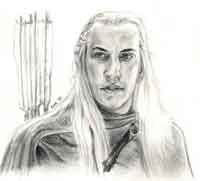
\includegraphics[width=0.4\textwidth]{elf.jpeg}

At that time forests spread across the lands and there were only a few human city states scattered around the Middle Sea.

The first Orcish Raid recorded by the Elves occurred circa AUC -2000.  It was easily repelled by the highly disciplined Elvish armies.  However the repeated raids from Orcish Hordes gradually eroded the strength of the Fëanorian Legions.  

Their numbers grew few and they lost confidence they could hold the orcs off for much longer.  The Elves aware of the approaching fall of their empire, despaired for their nation and their children.  Some elves turned to the worship of the Great Old Ones hoping to be saved by divine intervention.


In AUC -1553, the Hordes of Gorosh the Mighty marched into what is now present day Brythinia.  Their numbers so great it was said that they were beyond counting.  Aurelion Hightower, King of Kings, led the armies of the elves against the Orcish multitude. 

 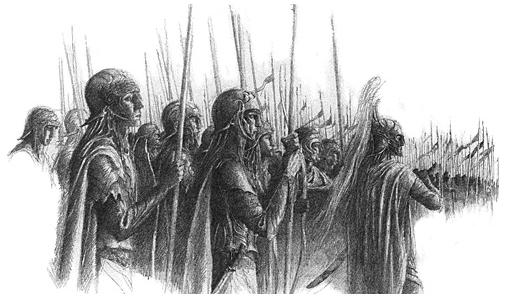
\includegraphics[width=0.4\textwidth]{legion.jpg}

They fought for seven days until the apostates, despairing for their own lives, used blood magic to attempt to open a gate to one of the outer dimensions.  Hoping that by sacrificing the lives of their bretheren they could save their own, the heretical regiments attacked the serried array of the elven army in the flank.  From this they gained much power and it is said that the gate they opened, using the magical potential from the deaths of their fallen brothers, was so large that it filled the sky.  The land became deathly cold and dark.  Aurelion seeing this new danger charged the regiments of the heretics.  He road down the renegades for his heart was filled with honour and duty while theirs was filled with fear and self-loathing.  The gate was closed as the instigators of the fell magic were slain but not before many creatures were released upon the battlefield and many in the armies on both sides were malformed in horrific ways, twisted by the inscrutable whim of those beyond.  

Aurelion managed to drive off Gorosh's army though he was fatally wounded.  Shortly thereafter Gorosh was murdered by his generals.  The apostates, who now called themselves the Druchii, fled North to the land of ice, dread Nagaroth, to avoid punishment for their crimes.  The last great elvish empire had been broken upon Orcish spears and the blades of those they trusted.

\begin{flushright}
 \includegraphics[width=0.4\textwidth]{dark_elves.png}
\end{flushright}
  

In the years that followed, a time known as the Sundering, there was a brief civil war.  The elvish nation split into factions in the north around Hibernia, Cheruskia and Brythinia and in the south around Averoigne and Aquillonia.  Those elves of the north, later deciding that it was indefenisble, withdrew from Brythinia.

Circa AUC -1500 the remnants of the Fëanorian empire collapsed, its power having being eroded by ceaseless waves of orcish raiders. The great fecundity of the Orcs being the decisive factor in the stuggle.  The Orcs succeeding where hundreds of other threats had failed.  Satelite states abandonded the elves.  Human nations expanded into the power void left by the collapsing elvish states.

Those elves in the north became the Namorian elves or Wood Elves, living in the forests around Iron Hills.  Those in the south found safe haven in the Sylvannian forests. 

 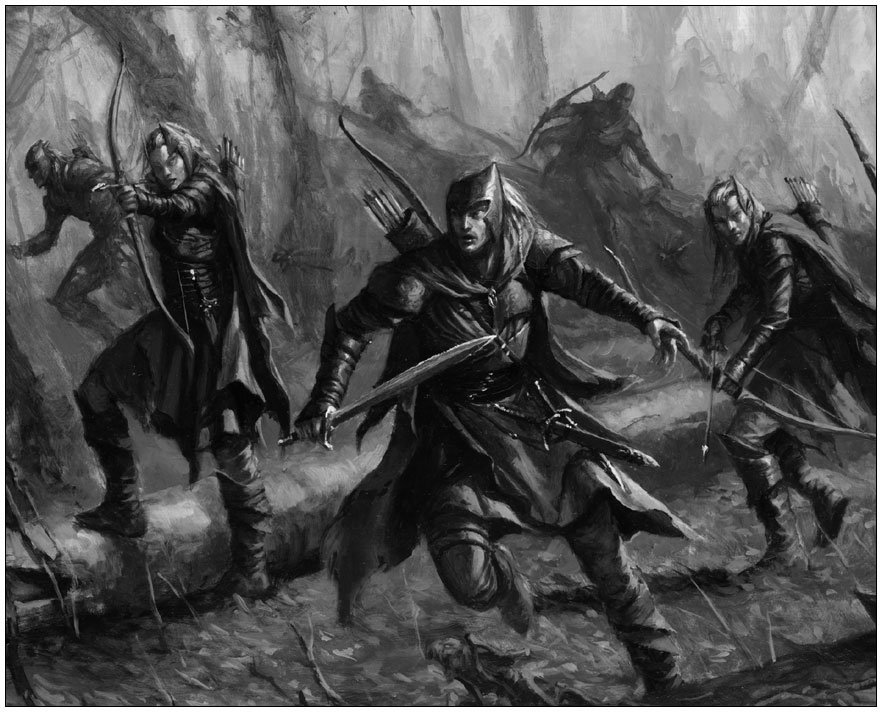
\includegraphics[width=0.4\textwidth]{wood_elf.jpg}

Wood elves hold themselves above all other races treating them with disdain.  Fighting many wars with their neighbours.  The wood elves are an insular race, largely keeping to themselves.  They trade for metal and some exotic foods but are largely self-sufficent.  Their small communities are usually situated in glades or suspended above the forest floor.  

 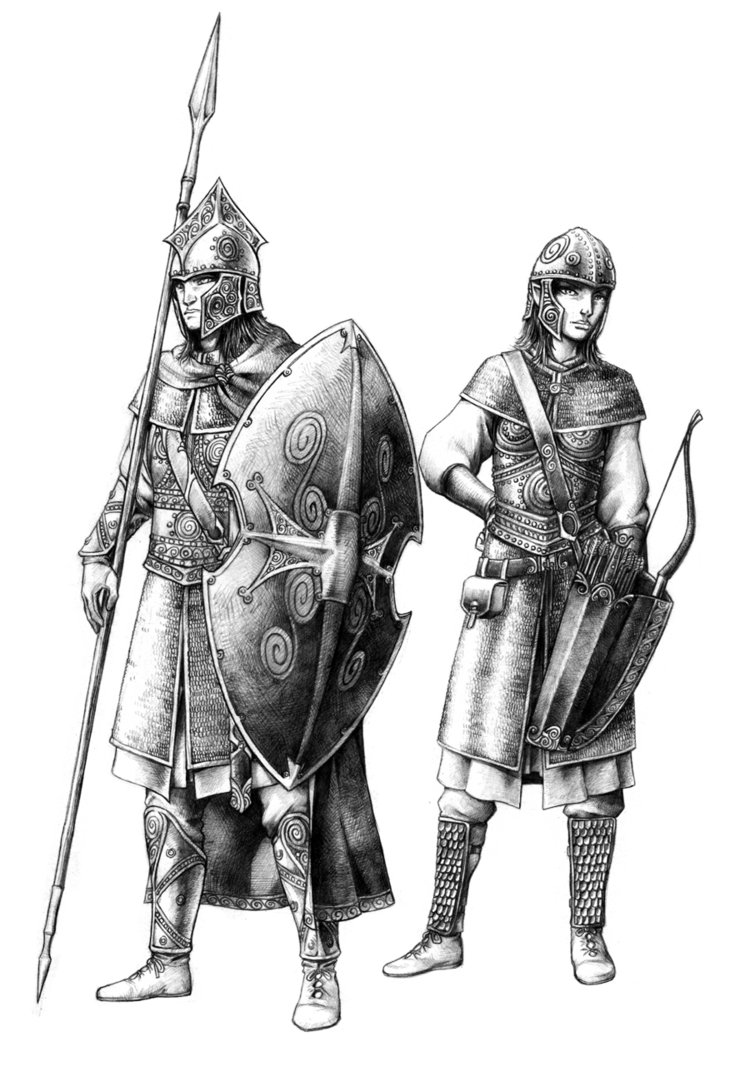
\includegraphics[width=0.4\textwidth]{high_elves.png}

The High Elves  live in many spired fortified cities made of marble amongst the forests of Sylvannia.  There they pursue academic interests or pursue political power in the high council or by convoluted political affairs with foreign powers.  The High Elves refuse to acknowledge in public that their empire is no longer.  They view other races and nations as being ungrateful and traitorous upstarts.  The Aquillonian empire regarded the academic achievements of the elves in high regard.  It's presence has sheltered them from dangers for two millenia.

 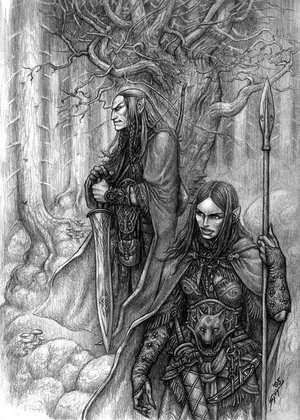
\includegraphics[width=0.4\textwidth]{dark_elf_raiders.jpg}

There is no apparent physical difference between the various groups of elves.  It is said that their skin is fairer than the sun to look at. The only way to tell them apart is by their dress, their mannerisms, accent etc.  Because of this and the behaviour of the Druchii elves are shunned throughout the north.  The followers of Caiphon are also prominent in promoting distrust of the elves.


\end{document}


